\section{\benchmarkname}
\label{sec: dataset}
% As illustrated in Figure~\ref{fig: annt_pipeline}, w
We design a three-stage annotation pipeline for the construction of our benchmark. The three stages will be introduced in Section~\ref{subsec: document collection}, Section~\ref{subsec: qa collection}, and Section~\ref{subsec: quality control}, respectively. We also provide key statistics of our benchmark in Section~\ref{subsec: dataset_overview}.

% \begin{figure}[!htbp]
%     \centering
%     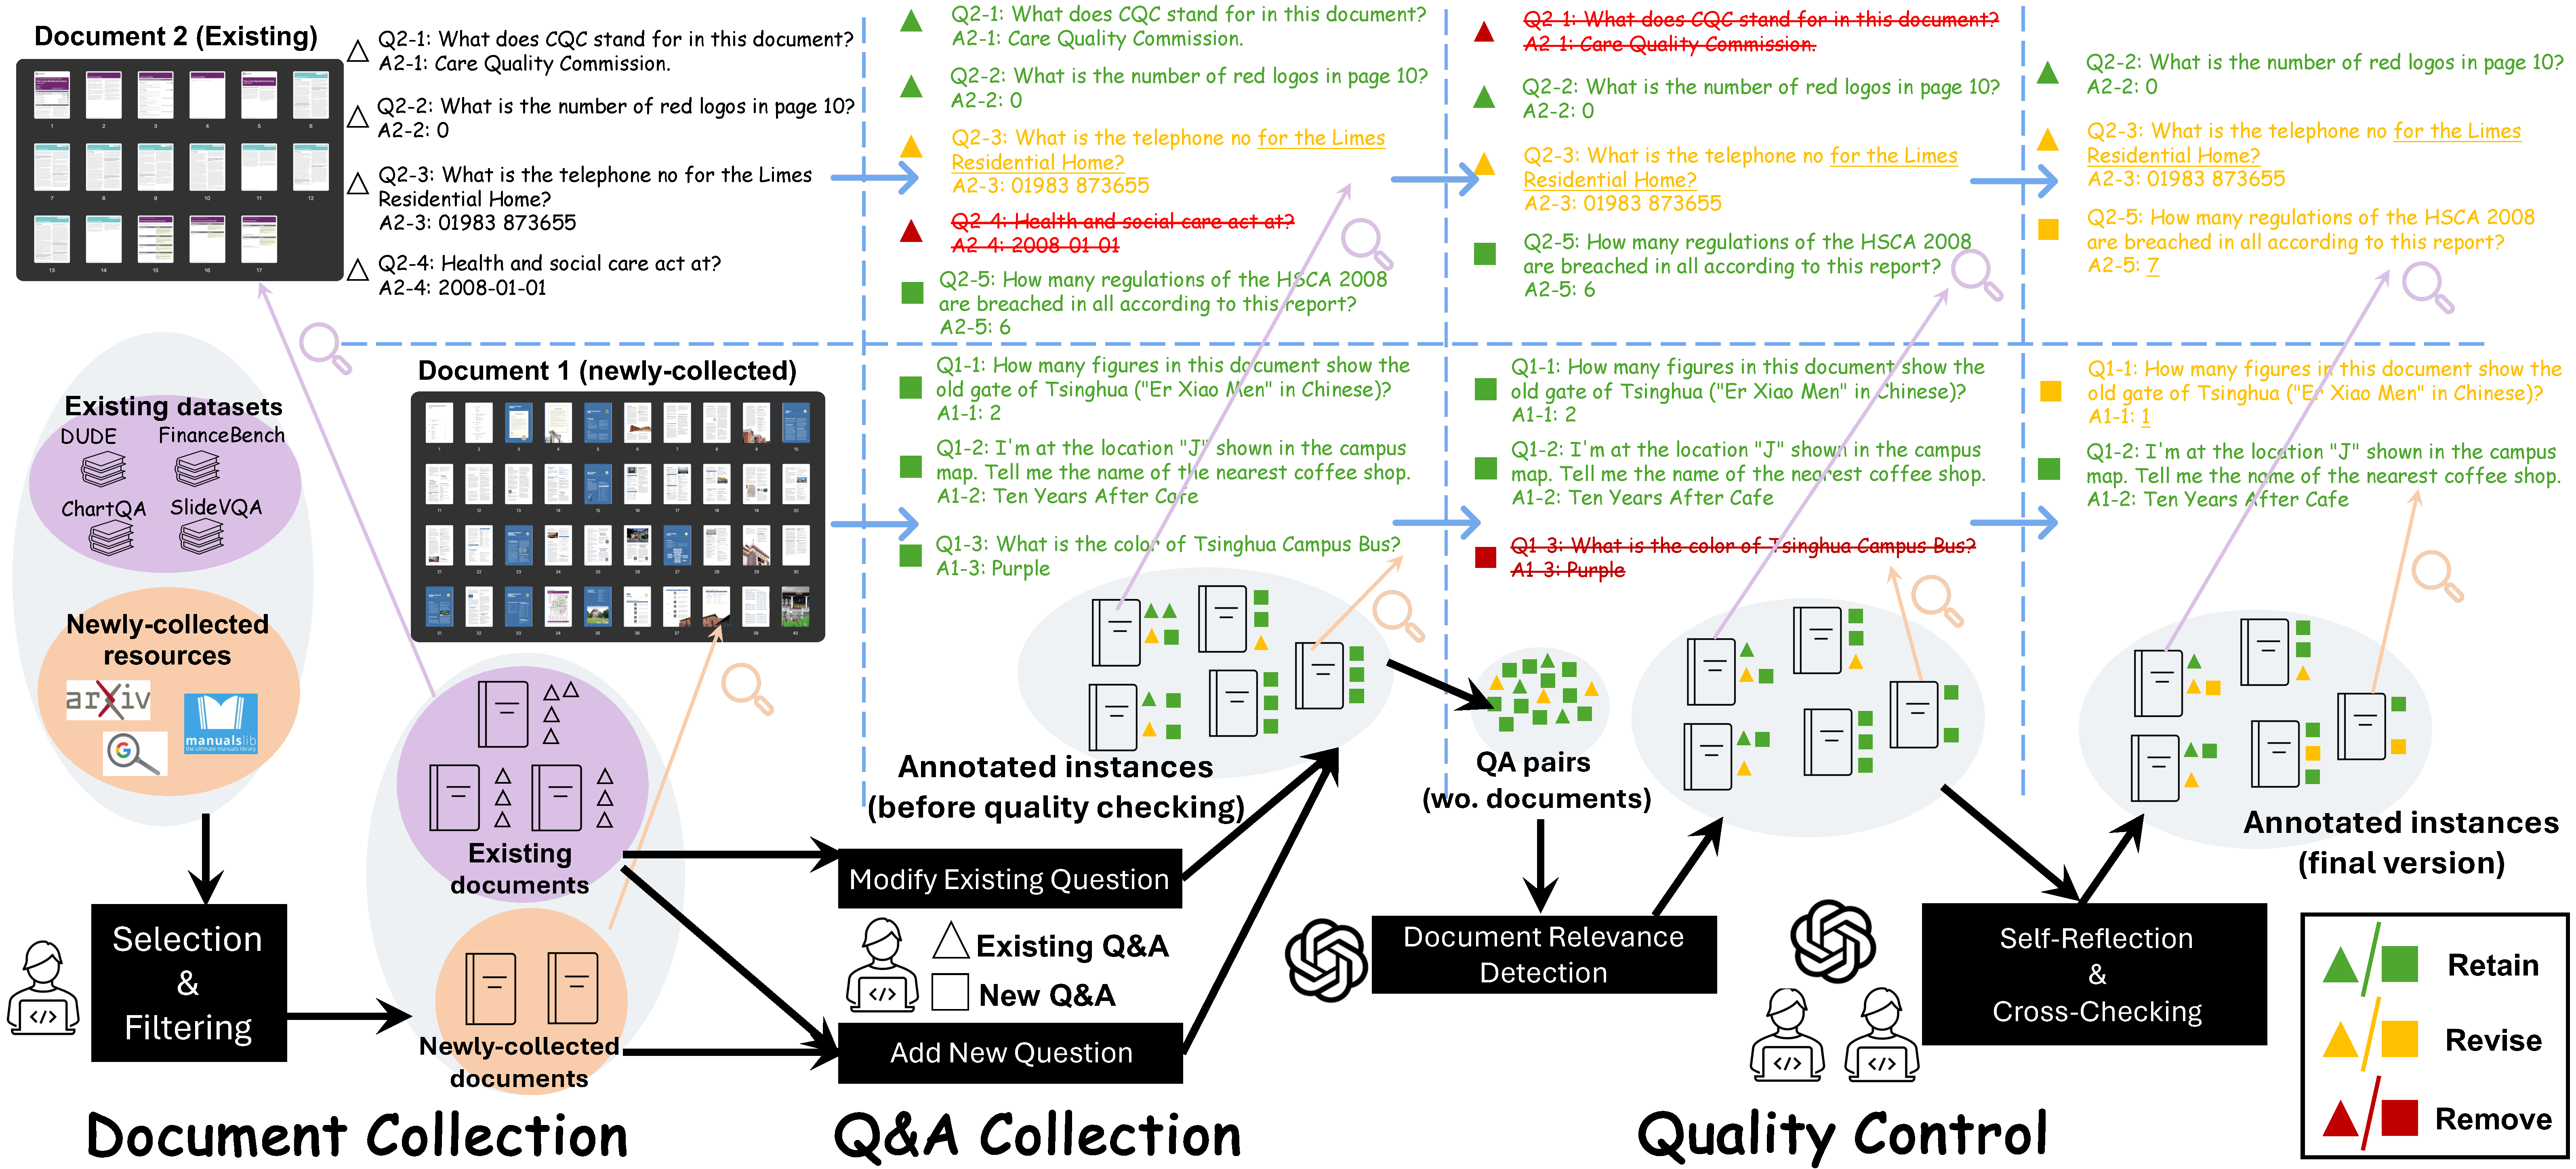
\includegraphics[width=\textwidth, bb=0 0 3061 1389]{figures/annotation_pipeline.pdf}
%     \caption{The annotation pipeline of \benchmarkname.}
%     \label{fig: annt_pipeline}
% \end{figure}

\subsection{Document Collection}
\label{subsec: document collection}
As a long-context DU benchmark, the documents shall be of diverse topics and lengthy enough. To this end, we crawl a great amount of documents from various sources. Then we select the lengthy ones from these documents. Specifically, we encompass a diverse array of documents from two approaches. (1) \textbf{Existing documents} from four previous datasets: DUDE~\cite{VanLandeghem2023DocumentUD}, SlideVQA~\cite{SlideVQA2023}, ChartQA~\cite{masry-etal-2022-chartqa}, and FinanceBench~\cite{islam2023financebench}. (2) \textbf{Newly-collected documents} from Arxiv~\footnote{\texttt{https://arxiv.org}}, ManualsLib~\footnote{\texttt{https://www.manualslib.com}} and Google Search~\footnote{\texttt{https://www.google.com.sg}}. Then we (1) filter out the documents with fewer than 15 pages or license restrictions and (2) down-sample documents from DUDE, SlideVQA, and FinanceBench for a more balanced distribution. Detailed descriptions of our selection and processing procedure can be found in Appendix~\ref{appendix: Existing Document Collection} and Appendix~\ref{appendix: Newly-annotated Document Collection}.

In summary, we collect a total of 135 documents. Among them, 76 documents are from existing datasets 
% (colored in purple and exemplified as Document 2 in Figure~\ref{fig: annt_pipeline}, the same below) 
and incorporate previously annotated questions (represented as triangles). The remaining 59 documents are newly collected 
% (colored in orange and exemplified as Document 1) 
and incorporate no existing questions. We manually categorize them into 7 types: \textit{Research Report}, \textit{Financial Report}, \textit{Academic Paper}, \textit{Brochure}, \textit{Guideline}, \textit{Administration \& Industry File}, \textit{Tutorial / Workshop}. We showcase some instances of these documents in Appendix~\ref{appendix: Document Examples}.


\subsection{Question and Answer Collection}
\label{subsec: qa collection}
To serve as a high-quality and comprehensive benchmark, the question annotation of our benchmark adheres to the following standards: (1) All questions shall be neither over-easy nor over-difficult. (2) Questions are not repetitively derived from the same page or the same pattern. (3) The distribution of evidence numbers, evidence sources, and evidence locations for the questions shall be balanced. (4) No questions shall be answered correctly without accessing the relevant documents. 

Ten authors serve as expert-level annotators for the question-and-answer collection. All of them are doctors or Ph.D. students proficient in English reading and writing. Before formal annotation, they undergo a training session and pre-annotate three documents for practice. We iteratively review their annotation results and provide personalized feedback until their annotations meet the standards mentioned above. Regarding the formal annotation, we divide 135 documents into 54 batches (each having 2-4 documents) and dispatch these batches to annotators. We then ask the annotators to submit their results in units of batches and set reasonable time intervals for each batch's submission. We timely evaluate their annotations after each submission and remind the annotators if their questions in this turn diverge from the standards. It avoids the annotators rushing all assignments in a short time and benefits the annotation quality. We recommend the annotators take 60-90 minutes on each document. Specifically, the annotators shall rapidly read through the whole document in the first 15-30 minutes. For the remaining time, they shall dive deep into specific components to modify existing annotations and/or add new annotations as detailed below.

\noindent \textbf{Modify Existing Questions.} 
Documents collected from existing datasets had been annotated with some questions and answers from previous work. However, their crowd-sourcing annotations inevitably make some questions, answers, and other meta information unqualified. Therefore, we edit their annotations before including them as a component of our benchmark.

Specifically, we classify six potential problems in original annotations: \textit{Wrong Answers or Evidence Pages}, \textit{Repetitive Question}, \textit{Ambiguous Question}, \textit{Decontextualization-required Question}, \textit{Low Document-relevant Question} and \textit{Potential Shortcut}. See detailed explanations and examples about these problems in Appendix~\ref{subsec: Existing Question Editing}. Given an existing document, the annotators are tasked to evaluate each existing question's quality according to whether they have one or more above problems and assign a label from \{\texttt{Retain}, \texttt{Revise}, \texttt{Remove}\} for each question. Then the annotators would revise the \texttt{Revise} questions to meet our quality criteria and remove the \texttt{Remove} questions. 
% See triangle-marked questions colored in green, yellow, and red in Figure~\ref{fig: annt_pipeline} as \texttt{Retain}, \texttt{Revise}, \texttt{Remove} examples, respectively. 
Among all 425 original questions from 76 existing documents, 32.2\% of them are revised and 46.1\% are removed. We finally collect 211 questions in this procedure. The corresponding GUI is shown in Appendix~\ref{appendix: GUI Screenshots}.


\noindent \textbf{Add New Questions.} 
We newly annotate questions on both existing and newly collected documents to expand the questions in our benchmark. 
% See square-marked questions in Figure~\ref{fig: annt_pipeline} as examples. 
Specifically, we ask annotators to add about 3 questions on existing documents, and 6 questions on newly-collected documents. Given most existing questions (even after editing) are single-page ones and sourced from texts, we put more focus on (1) cross-page and unanswerable questions and (2) questions sourced from tables, charts, and images for newly added questions to balance the distribution. We detail the quantitative requirements in Appendix~\ref{appendix: New Question Annotation}. Associated with questions, annotators also provide reference answers and meta-information (\ie evidence sources, answer format, evidence locations) for all samples. We finalized a collection of 965 samples in this procedure. The corresponding GUI is shown in Appendix~\ref{appendix: GUI Screenshots}.

\subsection{Quality Control}
\label{subsec: quality control}

Combining the merits of humans and LVLMs, we adopt a three-round, semi-automatic quality control procedure to improve the annotation quality of our benchmark. We detail each round in the following components and leave the discussion of potential bias in Appendix~\ref{appendix: potential_bias}.

\noindent \textbf{Document-relevant Detection.} Our benchmark is designed to evaluate LVLMs' long-context document understanding abilities. All questions are expected to be unanswerable without access to corresponding documents. To remove low document-relevant questions (\ie questions not relying on documents), we feed each annotated question \textbf{WITHOUT} documents to GPT-4o. A question will be identified as \textit{low document-relevant} question if GPT-4o correctly predicts under this case. Ultimately, 94 samples are identified as low document-relevant questions and removed in this round.

\noindent \textbf{Self-reflection.} We draw inspirations from MMBench~\cite{mmbench2023} and leverage LVLMs to reduce the wrongly-annotated samples. Specifically, we feed the remaining questions from the last round \textbf{WITH} their documents to GPT-4o. Samples whose model predictions are inconsistent with the reference answers are sent back to corresponding annotators. The annotators are asked to check each question and identify whether the inconsistency is caused by \textit{problematic annotation} or not. As a result, 13.8\% of the samples are identified as problematic annotations. The annotators revise them accordingly.

\noindent \textbf{Cross-checking.}
In parallel, annotators cross-check the annotated samples from other annotators and determine the inconsistency reasons the same as described above. We calculate Cohen’s kappa value of their identifications as 0.42 (17.5\% inconsistent samples), showing a moderate agreement. Regarding the 17.5\% inconsistent samples, two primary authors serve as meta-annotators and make final decisions on them (and if necessary, revise accordingly).

\begin{figure}[htbp!]
 \begin{minipage}{0.5\textwidth} 
 \centering
 \fontsize{8.2pt}{\baselineskip}\selectfont % font size
 \renewcommand\tabcolsep{2.2pt} % column space
 \renewcommand\arraystretch{0.8} % row space
 \begin{tabular}{lc}
 \toprule
 \textbf{Statistic} & \textbf{Number} \\
 \midrule
  \textbf{Documents} & 135 \\
  ~- Type & 7 \\
  ~- Average/Medium pages &  47.5 / 28 \\
  ~- Average/Medium length & 21,214.1 / 12,179 \\
 \midrule
  \textbf{Total questions} & 1,082 \\
  ~- Single-page question & 494 (45.7\%) \\
  ~- Cross-page questions & 365 (33.7\%)  \\
  ~- Unanswerable questions & 223 (20.6\%) \\
 \midrule
  ~- Derived questions & 184 (17.0\%) \\
  ~- Newly-annotated questions & 898 (83.0\%) \\
\midrule
  (Evidence source) \\ 
  ~- Pure-text & 305 (35.5\%) \\
  ~- Layout & 119 (13.9\%) \\
  ~- Table & 218 (25.4\%) \\
  ~- Chart & 178 (20.7\%) \\
  ~- Image & 304 (35.4\%) \\
 \midrule
(Answer Format) \\ 
  ~- String   & 250 (29.1\%) \\
  ~- Integer  & 299 (34.8\%) \\
  ~- Float & 159 (18.5\%) \\
  ~- List & 151 (17.6\%) \\
 \midrule
 Avg./Max. question length & 16.4 / 60 \\
 Avg./Max. answer length & 2.8 / 54 \\
 \bottomrule
 \end{tabular}
\captionof{table}{Dataset Statistics}
 \label{tab:statistics}
 \end{minipage} 
 \hfill
 \begin{minipage}{0.5\textwidth}
 \centering
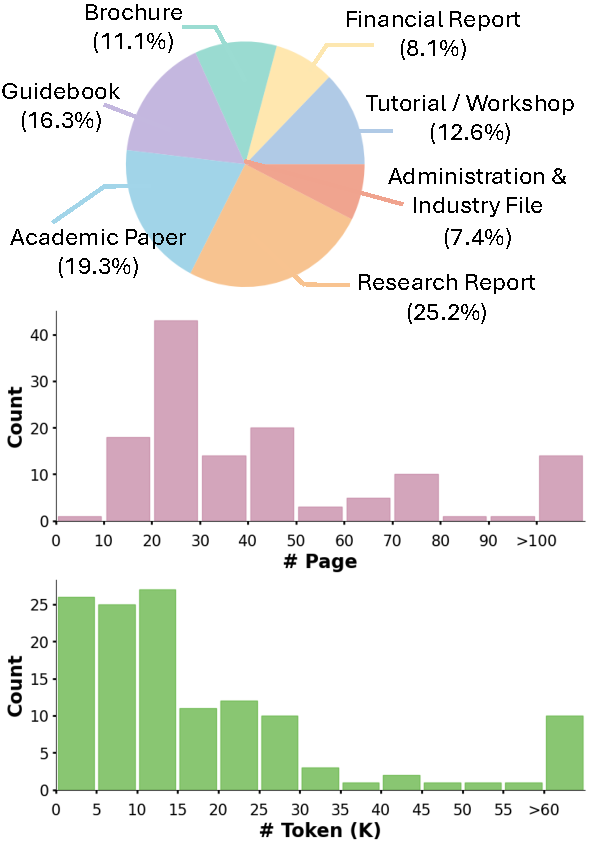
\includegraphics[width=0.8\linewidth, bb=0 0 284 411]{figures/statistics.pdf}
 \caption{Detailed distribution of documents. \textbf{Top}: Document type. \textbf{Middle}: Page Number. \textbf{Bottom}: Token Number.}
 \label{fig: document_distribution}
 \end{minipage}
\end{figure}

\begin{figure}[!htbp]
    \centering
    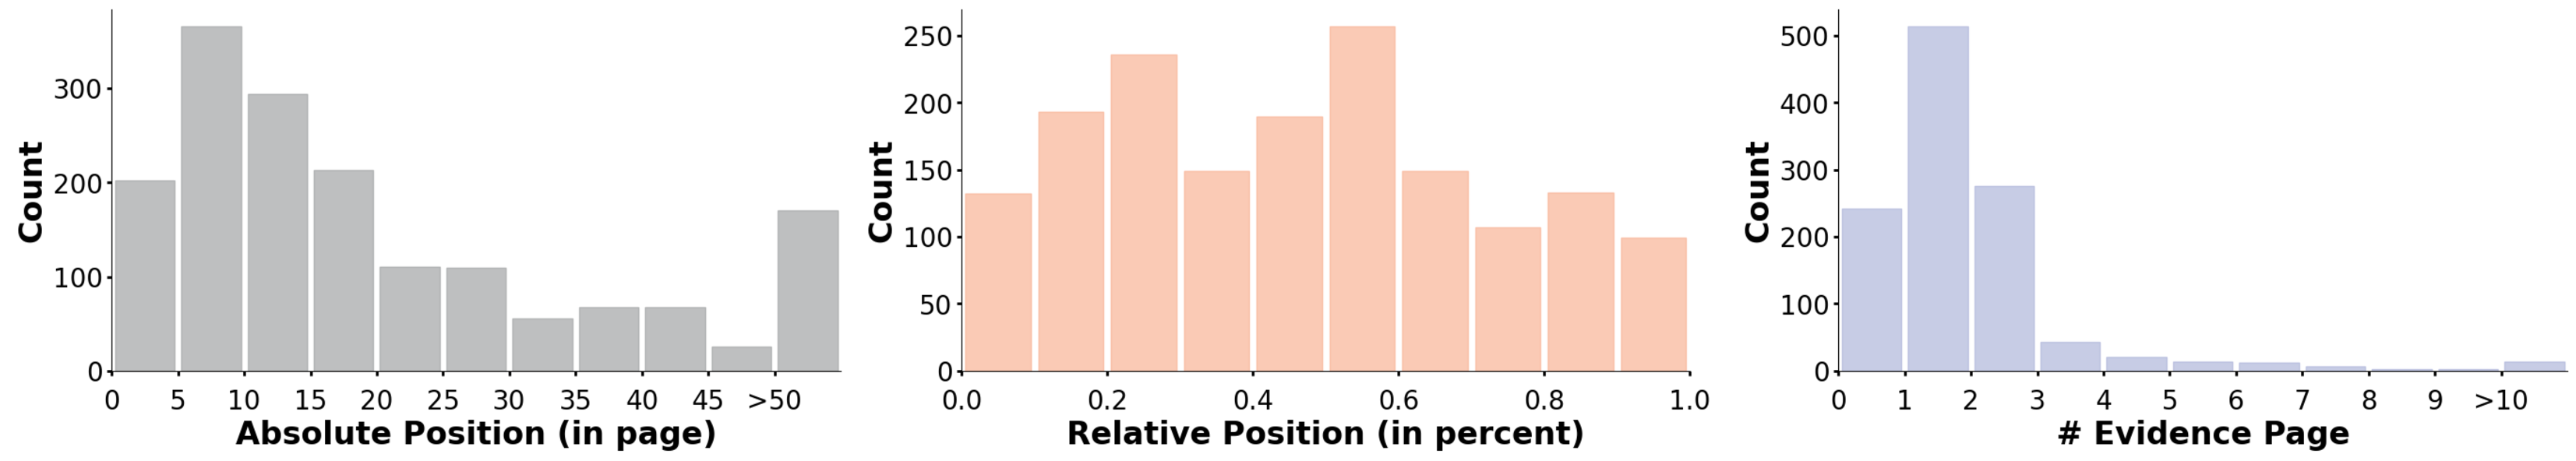
\includegraphics[width=\linewidth]{figures/question_statistics.pdf}
    \caption{Detailed distribution of questions \& answers. \textbf{Left}: Absolute position of answer evidences (the page index). \textbf{Middle}: Relative position (the page index/document page number). \textbf{Right}: Evidence page number of each question. (0: unanswerable question; >2: cross-page question).}
    \label{fig: question_distribution}
\end{figure}

\subsection{Dataset Overview and Analysis}
\label{subsec: dataset_overview}

The main statistics of \benchmarkname are presented in Table~\ref{tab:statistics}. Overall, our benchmark consists of 1,082 questions. These questions are constructed upon 135 lengthy documents across 7 document types, with an average of 47.5 pages and 21,214.1 tokens. Please see detailed distributions of these documents in Figure~\ref{fig: document_distribution}. Regarding the questions, there are 494 single-page questions (1 evidence page), 365 cross-page questions (2+ evidence pages), and 223 unanswerable questions (no evidence page). These three types of questions evaluate the LVLMs's long-context DU capabilities from complementary aspects: the localization ability, the cross-page comprehension ability, and the hallucination severity, respectively. For single-page and cross-page questions, their answer evidence is scattered among different context sources (\ie text, layout, table, chart, image) and evenly distributed across different locations of the documents (see Table~\ref{tab:statistics}, Figure~\ref{fig: question_distribution} Left and Middle). Also notably, 28.6\% of cross-page questions have more than two evidence pages, which further enhances the challenge of our benchmark.